\documentclass{beamer}
\usepackage[latin1]{inputenc}
\usetheme{Warsaw}
\usecolortheme{wolverine}
\title{Soldering Workshop}
\author{Clint Grimsley clint.grimsley@gmail.com}
\institute{HackRVA}
\date{August 13, 2012}
\begin{document}

\begin{frame}
\titlepage
\end{frame}

\begin{frame}
  \frametitle{Outline}
    \tableofcontents
\end{frame}

\section{Basics}
\subsection{Good}
\begin{frame}
  \frametitle{Good}
  \begin{columns}
    \begin{column}{5cm}
      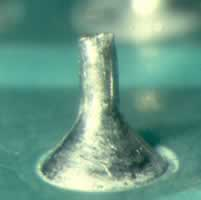
\includegraphics{images/good_joint.jpg}
    \end{column}
    \vspace{3cm}
    \begin{column}{5cm}
      \begin{itemize}
        \item blah
        \item blah2
      \end{itemize}
    \end{column}
  \end{columns}
\end{frame}
\subsection{Bad}
\begin{frame}
  \frametitle{Bad}
  
\end{frame}
\subsection{WTF?}
\begin{frame}
  \frametitle{WTF?}
  
\end{frame}
\section{Physics}
\subsection{Heat}
\begin{frame}
  \frametitle{Heat}
  Physics is how to make oneself comfortable handling a 750\textdegree F  iron and slinging molten lead around 

  Adages I follow:
  \begin{itemize}
    \item Heat the work, not the solder
    \item Too much Rosin is your mortal enemy
    \item Not enough Rosin is the mortal enemy of heat
  \end{itemize}
\end{frame}

\subsection{Gravity}
\begin{frame}
  \frametitle{Gravity}
  \begin{itemize}
    \item Understand the best way to mount your work, so your project
      doesn't crash to the floor and your components don't fall all
      over the place
    \item I usually accomplish this by resting the work against small
      odds and ends on the table
  \end{itemize}
\end{frame}

\section{References}

\begin{frame}
  These docs and their authors rock, and this presentation would have
  sucked more without them.
  \begin{itemize}
    \item \url{http://www.ami.ac.uk/courses/topics/0170_wsp/index.html}
    \item \url{http://pages.csam.montclair.edu/~west/phys240/Soldering.pdf}
  \end{itemize}
\end{frame}


\end{document}
